% PUMA TPC reconstruction — technical note. Compile: tectonic PUMA_report.tex
% Figures shared with the slide deck (./figs/).
\documentclass[11pt,a4paper]{article}
\usepackage[margin=2.4cm]{geometry}
\usepackage{graphicx,amsmath,amssymb,booktabs,siunitx,xcolor}
\usepackage[hidelinks]{hyperref}
\usepackage{caption}
\captionsetup{font=small,labelfont=bf}
\usepackage{sectsty}\sectionfont{\large}
\setlength{\parskip}{4pt}\setlength{\parindent}{0pt}

\title{\vspace{-1.2cm}\textbf{Reconstruction studies for the PUMA active-target TPC}\\[2pt]
\large A technical note: pulse analysis, pattern recognition and track fitting}
\author{Y.\ Ayyad \\ \small IGFAE / Universidade de Santiago de Compostela}
\date{\today}

\begin{document}
\maketitle
\vspace{-0.6cm}

\begin{abstract}\small
\noindent We document a full reconstruction chain for the PUMA active-target time-projection chamber
(annular P10 pad plane, \SI{4}{\tesla}), developed and validated on a native macOS build of
ATTPCROOT (ROOT 6.32 / FairRoot v19 / Geant4 11.2). Using a back-to-back $\pi^+\pi^-$ validation
channel we study each stage: (i) pulse-shape analysis with a fitted GET response; (ii) pattern
recognition, comparing four track finders and identifying \textbf{HDBSCAN} density clustering as the
most robust, decisively so for the same-charge, near-straight $K^+K^+$ topology; (iii) track fitting
with two independent Kalman filters (UKF, GENFIT). We reach a momentum resolution of
$\sim\!16\%$, an angular resolution of $\sim\!2^\circ$, sub-millimetre vertexing and $99.5\%$
charge identification. We further diagnose a momentum bias as energy loss in the Cu antiproton
trap and Al cryostat upstream of the gas, and remove it with a deterministic material correction
that keeps the bias within $\pm2\%$ from 150 to \SI{900}{MeV/c}. Finally, we show that the always-on
DLC resistive anode --- a liability with pad-centre reconstruction --- becomes a resolution
\emph{advantage} when its sub-pad charge is properly exploited (MultiFit + HDBSCAN + per-ring
charge-weighting): GENFIT then reaches an unbiased \textbf{7\%} momentum resolution, twice as good as
without DLC.
\end{abstract}

\section{Introduction}
PUMA measures low-energy antiproton annihilation on the surface of exotic nuclei; the charged
annihilation products ($\pi^\pm$, $K^\pm$) are tracked in an annular gas TPC inside a \SI{4}{\tesla}
solenoid. The pad plane is 16 equal-area rings $\times$ 256 azimuthal sectors (4096 pads,
$R=62.9$--\SI{121.1}{mm}); electrons drift over \SI{300}{mm} to the pads, giving $(x,y)$ from the
pad position and $z$ from the drift time. This note reports a complete simulation-to-tracks chain
and its performance on a back-to-back $\pi^+\pi^-$ channel (\SI{375}{MeV/c} nominal), used because
its known kinematics make every quantity a controlled measurement.

\section{Simulation and digitization}
Events are generated and transported in Geant4 11.2, ionization electrons are drifted and induced on
the pads (\texttt{AtClusterize}, \texttt{AtPulse}). The resistive DLC anode disperses charge with
$\sigma_{\rm DLC}=\sqrt{2t/(RC)}$; for the measured sheet resistance $R=1.2$--$1.5~\mathrm{M}\Omega/\square$
this gives $\sigma\approx1.0$--\SI{1.2}{mm}, spreading each cluster over $\sim$1--2 pads and raising
the pad multiplicity $\sim$4$\times$, which enables sub-pad centroiding.

\section{Pulse-shape analysis}
Each pad trace is fit with the GET electronics response,
$A\,e^{-3u}\sin(u)\,u^3$ with $u=(t-t_0)/\tau$ and $\tau=\SI{25}{TB}$
(\texttt{AtPSAMultiFit}). The fit reproduces the pulse shape essentially perfectly
(Fig.~\ref{fig:psa}). The fitted impulse time $t_0$ gives the \emph{unbiased} drift depth, while the
response peak lags $t_0$ by the $\sim$\SI{8.6}{mm} shaping delay. We verified that the three PSA
variants (peak / multi-fit-peak / multi-fit-impulse) are equivalent for momentum resolution
($\sim16$--$18\%$); the impulse-time option is preferable as it removes the shaping-delay $z$ offset
at the source. One fitted pulse yields one \texttt{AtHit}.

\begin{figure}[h]\centering
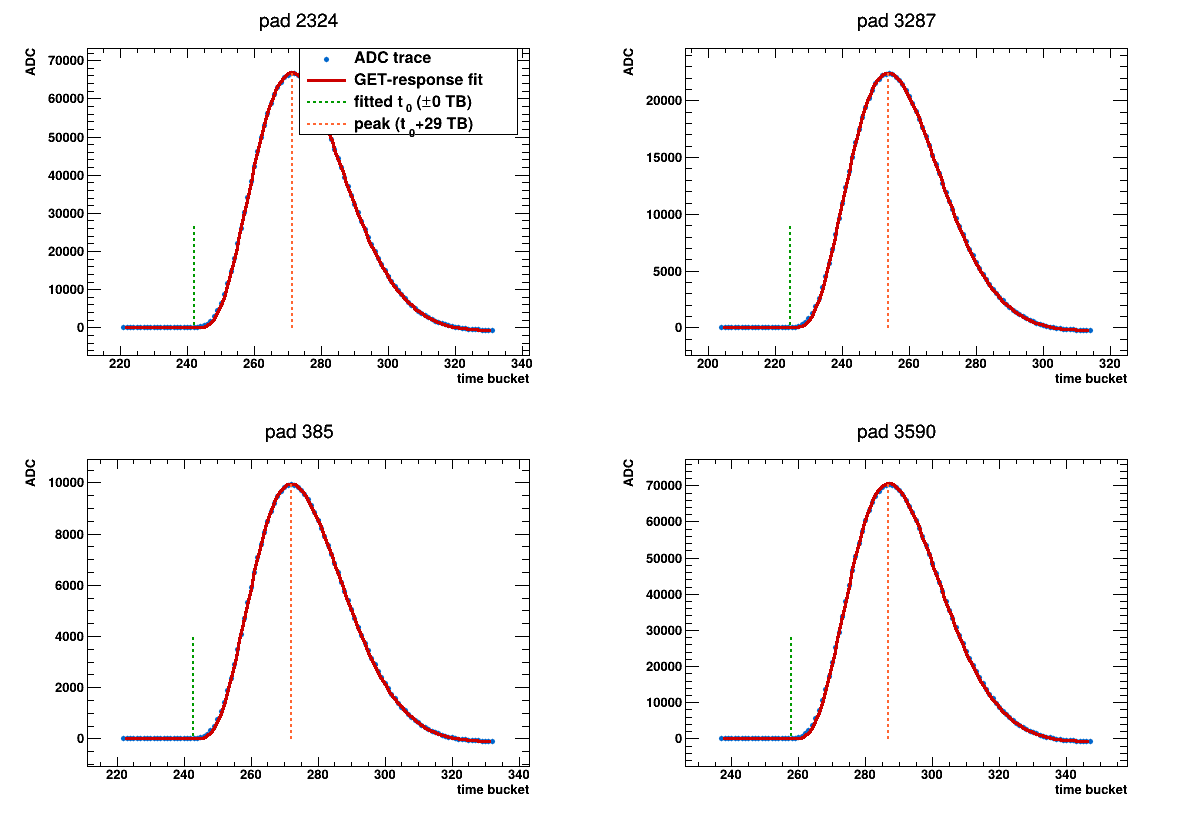
\includegraphics[width=0.86\linewidth]{figs/psa_fitshape.png}
\caption{GET-response fit (red) to four pad traces (blue). Fitted impulse time $t_0$ (green) and
response peak (orange) are marked. The fit tracks the pulse shape at all amplitudes.}
\label{fig:psa}
\end{figure}

\section{Pattern recognition}
Pattern recognition groups the \texttt{AtHit}s into track candidates. We compared four finders on
identical hits: two spatial-clustering methods (TriplClust, \texttt{AtTrackFinderTC}; and HDBSCAN
density clustering, \texttt{AtTrackFinderHDBSCAN}) and two global circle-consensus methods (Riemann,
RANSAC). Efficiency, purity and the fraction of cleanly reconstructed two-track events were measured
by hit-level truth matching.

\textbf{Clustering beats global fits.} On the two-pion channel the global circle fits fit one
dominant circle and merge the back-to-back pair ($\sim$50\% efficiency, $\sim$10\% clean events),
whereas spatial clustering finds both tracks ($99\%$ efficiency, $99\%$ purity, $86\%$ clean).

\textbf{Efficiency versus momentum} (Fig.~\ref{fig:praeff}, TriplClust) shows a clean sweet spot at
375--\SI{500}{MeV/c} ($\sim95\%$ clean events) bracketed by two failure modes: over-segmentation of
tightly-curled low-momentum tracks, and merging of near-straight high-momentum tracks.

\textbf{HDBSCAN is more robust} (Fig.~\ref{fig:praalgo}): it holds 83--90\% clean events from
375 to \SI{900}{MeV/c}, where TriplClust-default collapses. TriplClust can recover at high momentum
by lowering its cluster distance, but requires momentum-adaptive tuning that HDBSCAN does not.

\textbf{The decisive case} is the same-charge $K^+K^+$ final state at \SI{600}{MeV/c}: two
near-straight mirror-circle tracks. Here TriplClust merges 57\% of the pairs (33\% clean events),
while HDBSCAN separates them cleanly --- $99\%$ efficiency, $99\%$ purity, $89\%$ clean events,
$0\%$ merged (Fig.~\ref{fig:kaon}). This establishes HDBSCAN as the track finder of choice for PUMA.

\begin{figure}[h]\centering
\begin{minipage}{0.49\linewidth}\centering
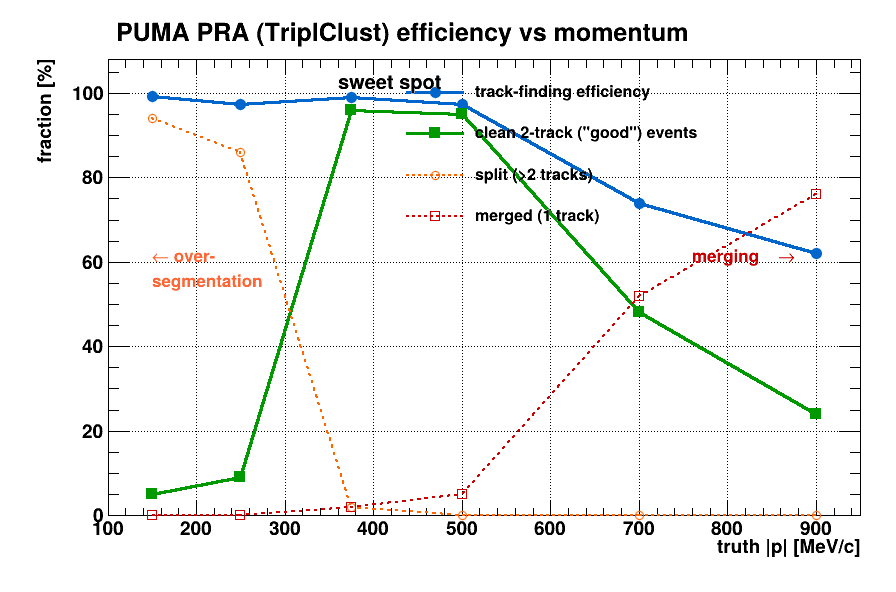
\includegraphics[width=\linewidth]{figs/pra_eff_vs_p.png}
\caption{TriplClust track-finding efficiency and clean-event fraction versus momentum.}
\label{fig:praeff}
\end{minipage}\hfill
\begin{minipage}{0.49\linewidth}\centering
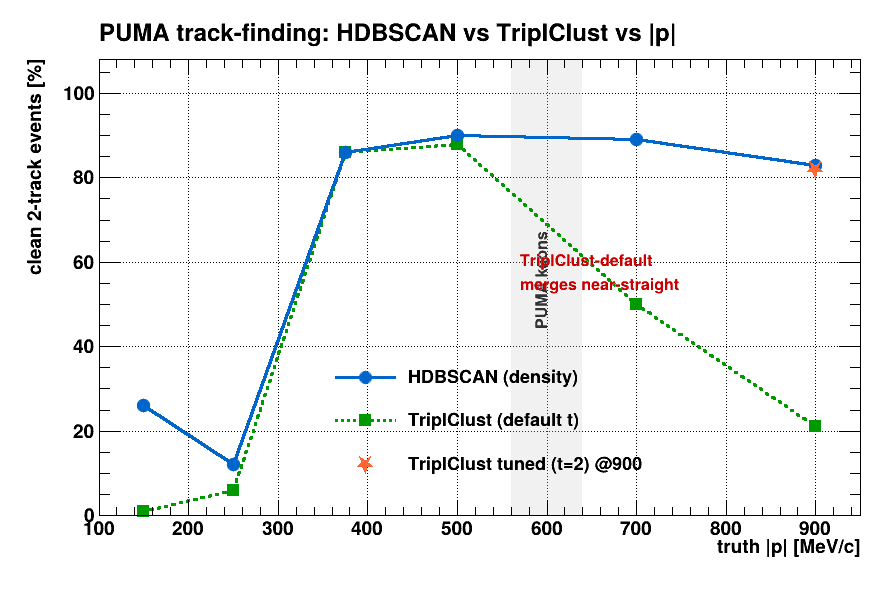
\includegraphics[width=\linewidth]{figs/pra_algo_vs_p.png}
\caption{Clean-event fraction: HDBSCAN vs TriplClust. HDBSCAN stays robust at high $p$.}
\label{fig:praalgo}
\end{minipage}
\end{figure}

\begin{figure}[h]\centering
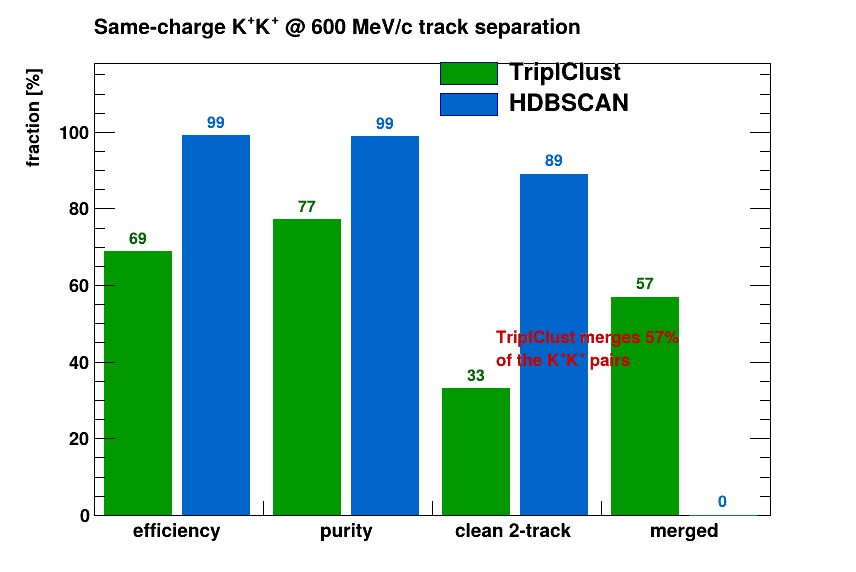
\includegraphics[width=0.66\linewidth]{figs/pra_kaon_cmp.png}
\caption{Same-charge $K^+K^+$ at \SI{600}{MeV/c}: HDBSCAN separates the near-straight mirror-circle
pair that TriplClust merges 57\% of the time.}
\label{fig:kaon}
\end{figure}

\section{Track fitting}
Each candidate is fit by two independent Kalman filters on the same clusters: an unscented Kalman
filter with CATIMA energy loss (UKF, \texttt{AtFitterUKF}) and a reference-track filter with native
Bethe-Bloch (GENFIT). Both back-extrapolate to the beam-axis vertex. On the $\pi^+\pi^-$ channel
(1000 events) the resolutions are summarised in Table~\ref{tab:res}; the UKF is the stronger fitter
on angle and vertex, the two are comparable on momentum, and charge identification is $99.5\%$ for
both. Fig.~\ref{fig:res} shows the momentum and vertex-$z$ residuals.

\begin{table}[h]\centering\small
\caption{Pion reconstruction efficiency and resolution (robust median/$\sigma_{\rm IQR}$),
1000 events at \SI{375}{MeV/c}. Tracking = true primaries found by pattern recognition;
fitting = PRA tracks successfully fitted.}
\label{tab:res}
\begin{tabular}{lcccccc}\toprule
 & tracking & fitting & momentum $\sigma$ & $\theta$ $\sigma$ & vertex $\sigma_z$ & charge-sign\\\midrule
UKF    & 99.6\% & 99.4\% & \textbf{16\%} & \textbf{2.1$^\circ$} & \textbf{0.62 mm} & 99.5\%\\
GENFIT & 99.6\% & 99.4\% & 18\% & 4.9$^\circ$ & 3.4 mm & 99.5\%\\\bottomrule
\end{tabular}
\end{table}

\begin{figure}[h]\centering
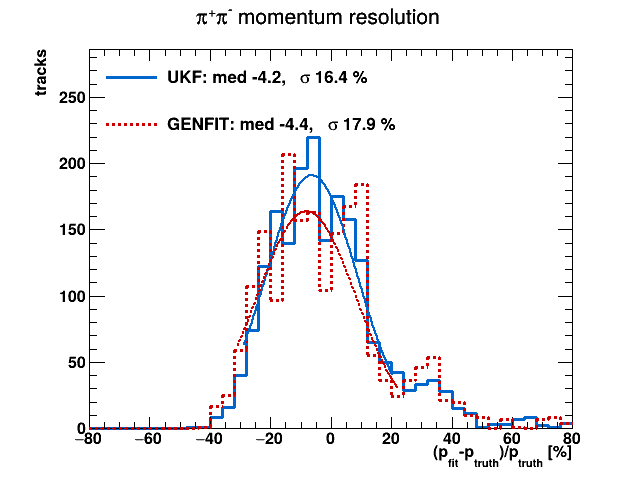
\includegraphics[height=4.6cm]{figs/res_pi_dp.png}\hfill
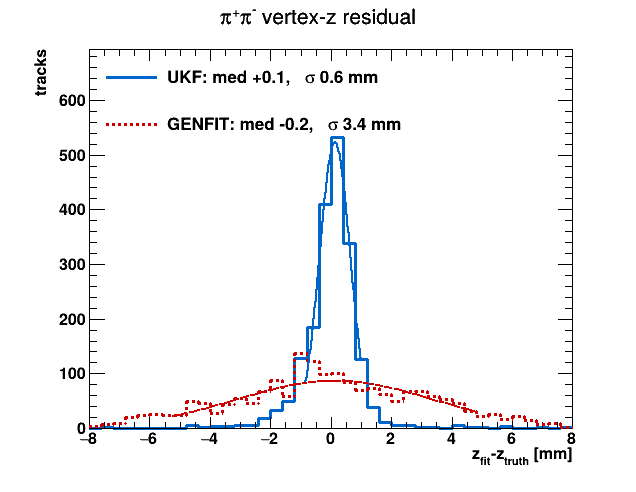
\includegraphics[height=4.6cm]{figs/res_pi_vz.png}
\caption{Momentum residual (left) and vertex-$z$ residual (right) for the two fitters, $\pi^+\pi^-$.}
\label{fig:res}
\end{figure}

\section{Momentum bias and the material correction}
The reconstructed momentum was initially biased low --- $-4\%$ at \SI{375}{MeV/c}, growing to $-20\%$
at \SI{150}{MeV/c}. This is \emph{not} a reconstruction error: the fit measures the in-gas momentum
correctly (residual $\lesssim1\%$ against the truth momentum entering the TPC). The annihilation
vertex sits inside a Cu antiproton trap ($R<\SI{10}{mm}$) and Al cryostat, and the pion loses
$\sim$\SI{16}{MeV} escaping to the gas \emph{before} it is tracked; the loss is larger at low
momentum (Bethe-Bloch). We remove it with a deterministic vertex material correction --- a single
reference offset scaled by the Bethe-Bloch $dE/dx\cdot(1/\beta)$ shape --- applied in both fitters.
The residual bias is then within $\pm2\%$ across 150--\SI{900}{MeV/c} (Fig.~\ref{fig:bias}).

\begin{figure}[h]\centering
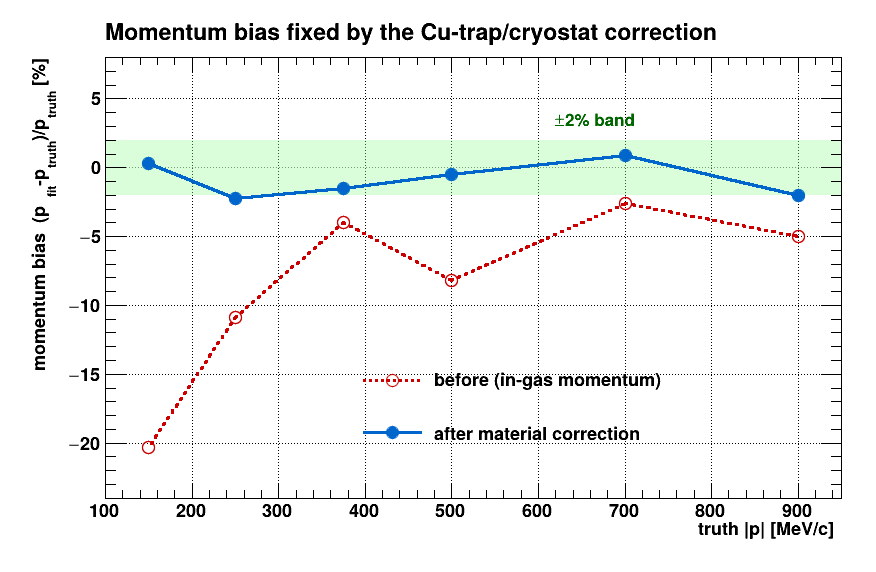
\includegraphics[width=0.62\linewidth]{figs/bias_fix.png}
\caption{Momentum bias versus $|p|$ before and after the Cu-trap/cryostat material correction.}
\label{fig:bias}
\end{figure}

\section{The DLC resistive anode: from liability to advantage}
The DLC anode is always active in the real detector, so its charge dispersion must be
reconstructed correctly. With the default chain it is a \emph{liability}: the $\sim$1.1\,mm
dispersion spreads each cluster over $\sim$4$\times$ more pads, and reconstructing them as
pad-centre hits (max-PSA) broadens the arc and biases the fitted circle radius low by $\sim$30\%
(a $-20\%$ momentum bias even with charge-weighted ring clustering; a blunt amplitude threshold does
not help --- it overshoots and destabilises).

\textbf{The cause is a reconstruction artefact, not physics.} The digitisation is faithful: the
deposited-charge centroid still marks the true trajectory. The bias is introduced downstream, when
max-PSA reduces each fired pad to a single hit at its \emph{geometric centre} and thereby discards
the sub-pad charge distribution. A track's ionisation, which physically lands at a well-defined
sub-pad point, is then represented by a $\sim$1--2 pad-wide band of pad-centre hits, and a
least-squares circle through that artificially broadened band returns a systematically smaller
radius --- hence a low momentum. The decisive evidence that this is a centroiding problem is that
the bias shrinks \emph{monotonically} as the charge-weighted centroid is recovered more accurately
($-30\% \to -20\% \to -9\% \to -6\%$, Fig.~\ref{fig:dlcladder}) and vanishes entirely once the
centroid is exact; and that the \emph{same} chain gives $\sigma=19\%$ without DLC but $\sigma=7\%$
with it --- the charge spread is what supplies the sub-pad information in the first place.

\textbf{The cure} recovers the true position as the charge-weighted centroid of each dispersed
cluster, and combines three ingredients
(Fig.~\ref{fig:dlcladder}): (i) \textbf{AtPSAMultiFit}, whose fitted pulse charge is a far better
per-pad weight than the peak ADC, halving the bias; (ii) \textbf{HDBSCAN}, which cleanly clusters the
dense dispersed band (TriplClust instead entangles the DLC bias with its own over-segmentation and
merging failure modes); and (iii) per-ring \textbf{charge-weighted centroiding}, which places one
sub-pad point per annular ring. With this chain the momentum resolution returns to the no-DLC value.

Crucially, \textbf{GENFIT} --- whose measurement model is told the ring centroids are accurate to
0.3\,mm --- exploits the sub-pad information fully: it becomes \emph{unbiased} and reaches a momentum
resolution of \textbf{7\%}, twice as good as the no-DLC case, and holds 7--9\% across the PUMA physics
range (375--\SI{600}{MeV/c}), while the UKF recovers only the no-DLC 15\% and keeps a small residual
bias (Fig.~\ref{fig:dlcukfgf}, Table~\ref{tab:dlc}). Properly reconstructed, the DLC anode is a
resolution \emph{advantage}, not a cost.

\begin{table}[h]\centering\small
\caption{Momentum reconstruction at \SI{375}{MeV/c} with DLC on, winning chain (HDBSCAN + MultiFit +
ring). GENFIT realises the sub-pad gain.}
\label{tab:dlc}
\begin{tabular}{lcccccc}\toprule
 & tracking & fitting & momentum bias & momentum $\sigma$ & $\theta$ $\sigma$ & vertex $\sigma_z$\\\midrule
UKF    & 99.7\% & 100\% & $-6.3\%$ & 15.1\% & 1.84$^\circ$ & 0.50 mm\\
GENFIT & 99.7\% & 100\% & \textbf{$-0.1\%$} & \textbf{7.1\%} & 1.76$^\circ$ & 0.47 mm\\\bottomrule
\end{tabular}
\end{table}

\begin{figure}[h]\centering
\begin{minipage}{0.47\linewidth}\centering
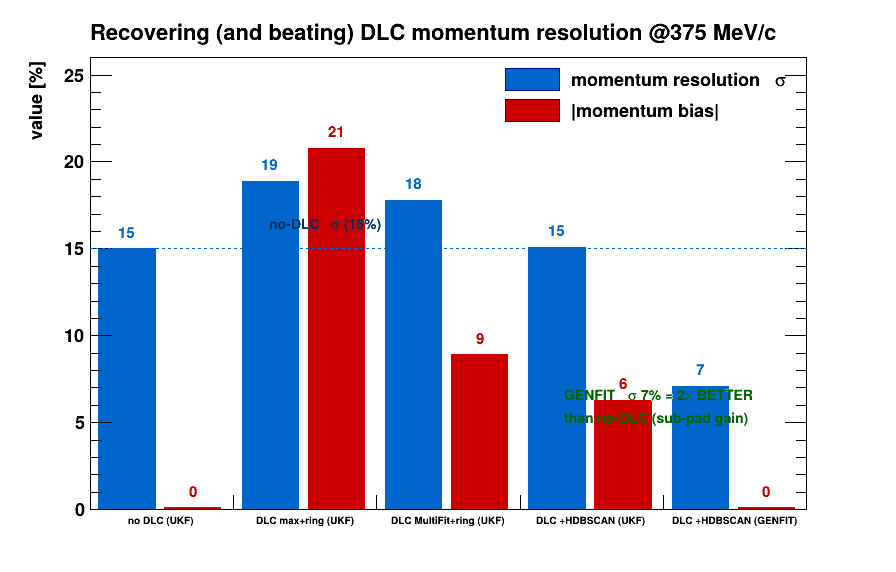
\includegraphics[width=\linewidth]{figs/dlc_ladder.png}
\caption{DLC momentum-recovery ladder at \SI{375}{MeV/c}: each reconstruction lever, ending with
GENFIT beating the no-DLC resolution.}
\label{fig:dlcladder}
\end{minipage}\hfill
\begin{minipage}{0.51\linewidth}\centering
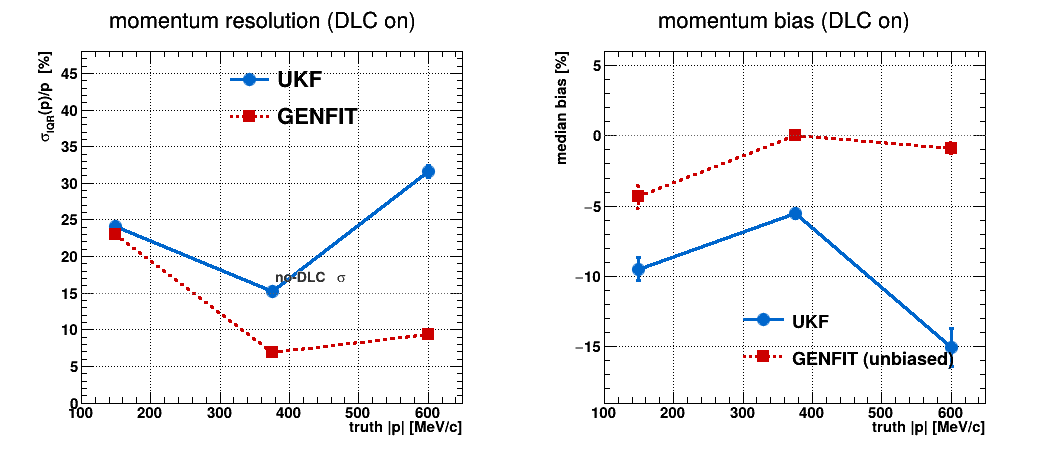
\includegraphics[width=\linewidth]{figs/dlc_ukf_genfit.png}
\caption{UKF vs GENFIT with DLC on (winning chain): resolution (left) and bias (right) vs $|p|$.
GENFIT is unbiased and $\sim$2$\times$ tighter.}
\label{fig:dlcukfgf}
\end{minipage}
\end{figure}

\begin{figure}[h]\centering
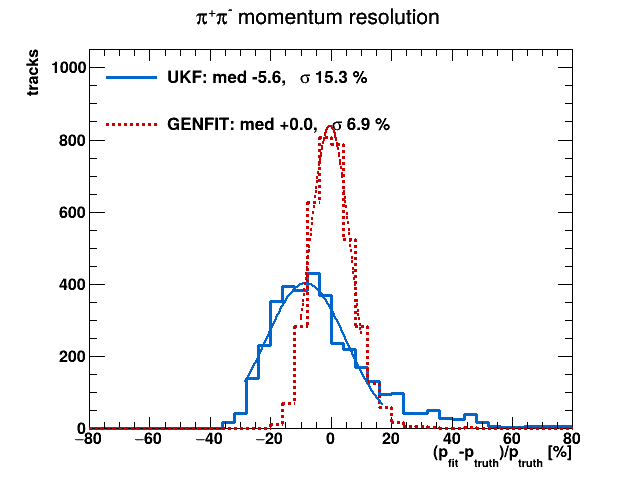
\includegraphics[width=0.56\linewidth]{figs/res_pi_dlc_dp.png}
\caption{Fully corrected momentum residual (winning chain, DLC on, 500 events): GENFIT peaks at
zero with $\sigma=7.2\%$, the UKF is broader ($\sigma=15\%$) and shifted ($-6\%$). This is the
final performance after both the Cu/Al material correction and the DLC sub-pad recovery.}
\label{fig:dlcres}
\end{figure}

\section{Particle identification}
$\pi^+$ and $\pi^-$ have identical mass and hence identical $dE/dx$; they are separated purely by
charge sign, i.e.\ signed magnetic rigidity $q\,B\rho=\mathrm{sign}\cdot p/0.2998$ [\si{\tesla\metre}].
Truth-labelled over 1000 events the two species form well-separated peaks (Fig.~\ref{fig:pid}) with a
charge identification of $99.5\%$ and a separation power $S=5.9\,\sigma$; the residual $\sim$0.5\%
cross-over is the mis-identification rate.

\begin{figure}[h]\centering
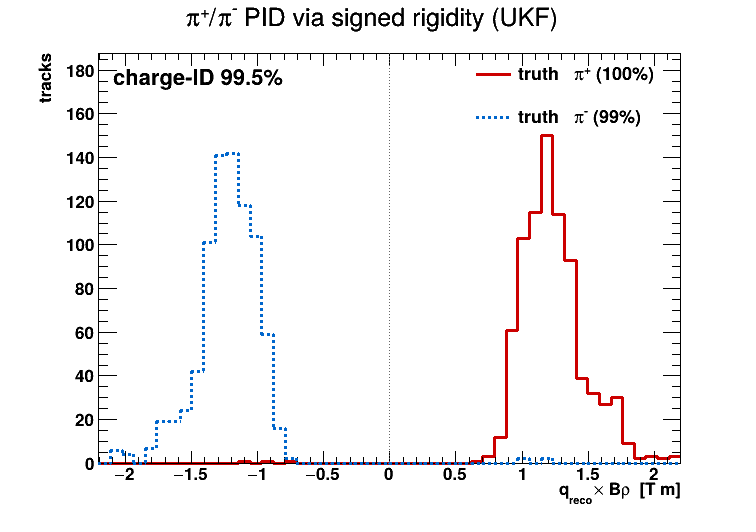
\includegraphics[width=0.56\linewidth]{figs/pid_pipm.png}
\caption{$\pi^+$/$\pi^-$ separation via signed rigidity. Charge-ID $99.5\%$, $S=5.9\,\sigma$.}
\label{fig:pid}
\end{figure}

\section{Summary and outlook}
A complete PUMA reconstruction chain --- simulation, DLC digitization, GET-response pulse analysis,
pattern recognition, and dual Kalman fitting --- runs natively on macOS and delivers
$\sim16\%$ momentum, $\sim2^\circ$ angular and sub-mm vertex resolution with $99.5\%$ charge-ID on
the $\pi^+\pi^-$ channel. The main methodological results are: HDBSCAN density clustering as the
robust track finder (decisive for the $K^+K^+$ topology); the equivalence of the PSA variants with a
preference for the unbiased impulse-time $z$; the identification and correction of the
upstream-material momentum bias; and, combining these, the recovery of the always-on DLC anode's
sub-pad information so that GENFIT reaches an unbiased $7\%$ momentum resolution --- twice as good as
without DLC. The recommended production chain is therefore \textbf{AtPSAMultiFit + HDBSCAN + per-ring
charge-weighted clustering + GENFIT} with DLC on. Natural next steps are the extension to the full
$K^+K^+\pi^-$ + hexaquark final state, a robustness study against electronic noise and pile-up, and
validation of the chain on a Linux build ahead of merging.

\end{document}
